\input{utils/preamble.tex}
\input{utils/macros.tex}

\title[Estimating Divergence Times]{Estimating Divergence Times}
\subtitle{Applied Phylogenetics}

\author[J.\ Oaks]{
    Jamie R.\ Oaks\inst{1}
}
\institute[University of Washington]{
    \inst{1}%
        Kincaid Hall 528 \hspace{1em} \href{mailto:joaks1@gmail.com}{\texttt{joaks1@gmail.com}}
}

% \date{\today}
\date{February 13, 2013}

\begin{document}

\maketitle

\begin{frame}
    \frametitle{Acknowledgements}

    Some of the slides and images are from a divergence-time
    \href{https://molevol.mbl.edu/wiki/images/6/6f/Bodega_2013_divtime_lecture.pdf}{lecture}
    by \href{http://phylo.bio.ku.edu/content/tracy-heath}{Tracy Heath}.
    
    \bigskip
    Thanks Tracy!
\end{frame}

\begin{frame}
\frametitle{Outline}
\tableofcontents
\end{frame}


\section{Why do we want to estimate trees with branches in units of time?}

\begin{frame}
\frametitle{Outline}
\tableofcontents[currentsection]
\end{frame}

\begin{frame}
    \frametitle{Why estimate divergence times?}
    \begin{itemize}
        \item Having a history of diversification through time is very powerful
        \item Have past environmental changes affected diversification?
        \item Epidemiology---Phylodynamics of pathogens
    \end{itemize}
\end{frame}

{
\usebackgroundtemplate{\includegraphics[width=\paperwidth]{../images/se-asia-present.png}}
\begin{frame}
    \frametitle{Southeast Asia}    
\end{frame}
}

{
\usebackgroundtemplate{\includegraphics[width=\paperwidth]{../images/se-asia-120.png}}
\begin{frame}
    \frametitle{Southeast Asia}    
\end{frame}
}

\section{Rates, time \& branch lengths}

\begin{frame}
\frametitle{Outline}
\tableofcontents[currentsection]
\end{frame}

\frame[plain]{\includegraphics[page=16,width=\textwidth]{../resources/Bodega_2013_divtime_lecture.pdf}}

\frame[plain]{\includegraphics[page=17,width=\textwidth]{../resources/Bodega_2013_divtime_lecture.pdf}}

\begin{frame}
    \frametitle{Rates and Time}
    \begin{itemize}
        \item We need to make some assumptions (i.e., create models)
            about the rate of evolution.
        \item By modeling how the rate of evolution behaves over time,
            we can tease apart rate and time and estimate branches
            \emph{proportional} to time
        \begin{itemize}
            \item Estimate \emph{relative} divergence times
        \end{itemize}
    \end{itemize}
\end{frame}


\section{Estimating relative divergence times}

\begin{frame}
\frametitle{Outline}
\tableofcontents[currentsection]
\end{frame}

\frame[plain]{\includegraphics[page=19,width=\textwidth]{../resources/Bodega_2013_divtime_lecture.pdf}}

\subsection{Modeling rates of evolution (``clock models'')}

\begin{frame}
\frametitle{Outline}
\tableofcontents[currentsection]
\end{frame}

\frame[plain]{\includegraphics[page=26,width=\textwidth]{../resources/Bodega_2013_divtime_lecture.pdf}}

\begin{frame}
    \frametitle{Global Molecular Clock}
    \begin{itemize}
        \item The simplest model
        \item We assume the rate of change is the same on every branch
        \item We explain long/short branches due to differences in time
        \item But \ldots
    \end{itemize}
\end{frame}

\begin{frame}
    \frametitle{Rates Vary!}
    What is a substitution?
    \begin{itemize}
        \item Mutations are introduced into a populations
        \item Some mutations fix to become substitutions
    \end{itemize}
    We expect the substitution rate to vary among lineages due to:
    \begin{itemize}
        \item Differences in underlying mutation rate
        \begin{itemize}
            \item Metabolic rates
            \item Generation times
            \item DNA repair mechanisms
        \end{itemize}
        \item Differences in selective constraints
    \end{itemize}
\end{frame}

\begin{frame}
    \frametitle{Rates Vary!}
    \begin{center}
        \includegraphics[width=0.8\textwidth]{../images/crocodylia-ml-tree.pdf}
    \end{center}
    We need ``relaxed-clock'' models to account for rate variation
\end{frame}

\frame[plain]{\includegraphics[page=34,width=\textwidth]{../resources/Bodega_2013_divtime_lecture.pdf}}
\frame[plain]{\includegraphics[page=38,width=\textwidth]{../resources/Bodega_2013_divtime_lecture.pdf}}
\frame[plain]{\includegraphics[page=39,width=\textwidth]{../resources/Bodega_2013_divtime_lecture.pdf}}
\frame[plain]{\includegraphics[page=69,width=\textwidth]{../resources/Bodega_2013_divtime_lecture.pdf}}
\frame[plain]{\includegraphics[page=70,width=\textwidth]{../resources/Bodega_2013_divtime_lecture.pdf}}
\frame[plain]{\includegraphics[page=74,width=\textwidth]{../resources/Bodega_2013_divtime_lecture.pdf}}
\frame[plain]{\includegraphics[page=32,width=\textwidth]{../resources/Bodega_2013_divtime_lecture.pdf}}
\frame[plain]{\includegraphics[page=33,width=\textwidth]{../resources/Bodega_2013_divtime_lecture.pdf}}

\begin{frame}
    \frametitle{Relaxed-clock models}
    \begin{itemize}
        \item There are a lot of models for rate variation over time
        \item By modeling rate variation, these relaxed-clock methods
            allow us to estimate trees with branches proportional
            to time
        \item What about absolute time?
    \end{itemize}
\end{frame}

\section{Estimating absolute divergence times}

\subsection{Calibrating rates of evolution}

\begin{frame}
\frametitle{Outline}
\tableofcontents[currentsection]
\end{frame}

\begin{frame}
    \frametitle{Calibrating rates}
    \begin{itemize}
        \item Sequence data are only informative on
            \emph{relative} divergences
        \item We need external information (like fossils) to
            calibrate (scale) the tree to absolute time
        \item A Bayesian statistical framework allows us
            to incorporate such information while accounting
            for uncertainty (priors!)
    \end{itemize}
\end{frame}

\frame[plain]{\includegraphics[page=86,width=\textwidth]{../resources/Bodega_2013_divtime_lecture.pdf}}
\frame[plain]{\includegraphics[page=87,width=\textwidth]{../resources/Bodega_2013_divtime_lecture.pdf}}
\frame[plain]{\includegraphics[page=88,width=\textwidth]{../resources/Bodega_2013_divtime_lecture.pdf}}
\frame[plain]{\includegraphics[page=89,width=\textwidth]{../resources/Bodega_2013_divtime_lecture.pdf}}
\frame[plain]{\includegraphics[page=101,width=\textwidth]{../resources/Bodega_2013_divtime_lecture.pdf}}
\frame[plain]{\includegraphics[page=102,width=\textwidth]{../resources/Bodega_2013_divtime_lecture.pdf}}
\frame[plain]{\includegraphics[page=103,width=\textwidth]{../resources/Bodega_2013_divtime_lecture.pdf}}
\frame[plain]{\includegraphics[page=105,width=\textwidth]{../resources/Bodega_2013_divtime_lecture.pdf}}
\frame[plain]{\includegraphics[page=106,width=\textwidth]{../resources/Bodega_2013_divtime_lecture.pdf}}
\frame[plain]{\includegraphics[page=107,width=\textwidth]{../resources/Bodega_2013_divtime_lecture.pdf}}
\frame[plain]{\includegraphics[page=108,width=\textwidth]{../resources/Bodega_2013_divtime_lecture.pdf}}
\frame[plain]{\includegraphics[page=109,width=\textwidth]{../resources/Bodega_2013_divtime_lecture.pdf}}
\frame[plain]{\includegraphics[page=110,width=\textwidth]{../resources/Bodega_2013_divtime_lecture.pdf}}

\begin{frame}
    \frametitle{Fossil calibrations}
    \begin{center}
        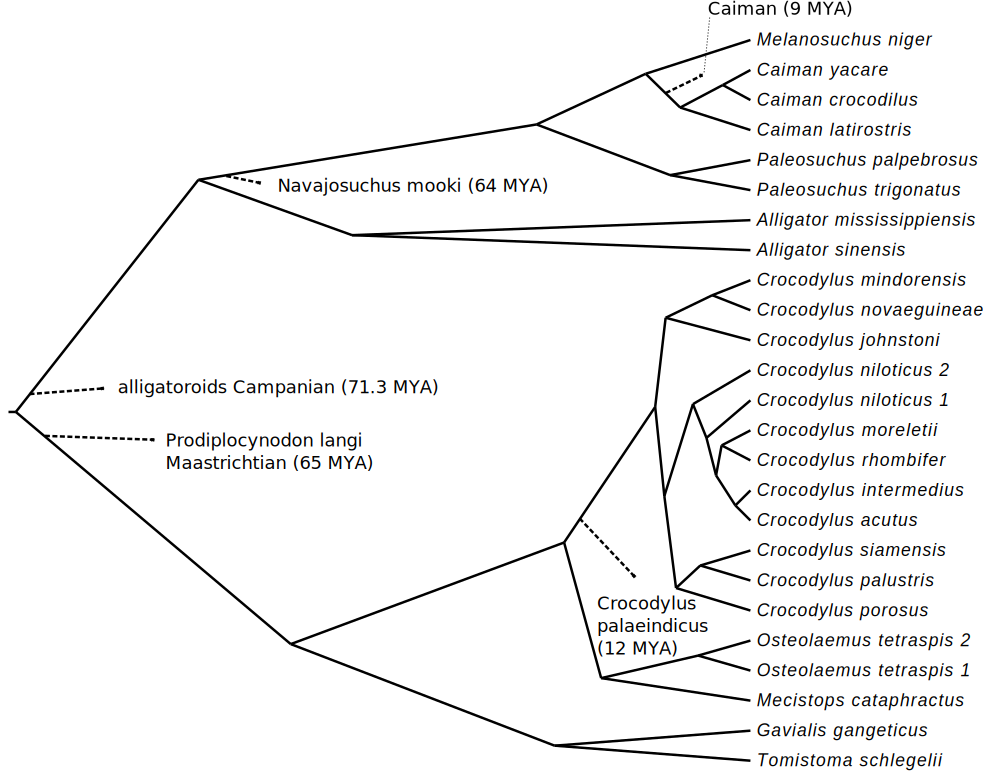
\includegraphics[width=0.8\textwidth]{../images/crocodylia-fossils.pdf}
    \end{center}
\end{frame}

\begin{frame}
    \frametitle{Fossil Calibrations---an issue}
    \begin{itemize}
        \item We are mixing priors on node ages!
        \item There is a prior on the tree and its branch
            lengths (e.g., birth-death process)
        \item We are adding additional priors on node ages
            based on fossils
        \item The resulting \emph{marginal} prior might not
            be what we expect!
        \item This is currently a ``hot'' area of research
    \end{itemize}
\end{frame}

\begin{frame}
    \frametitle{Fossil Calibrations---an issue}
    Potential solutions
    \begin{itemize}
        \item Incorporating fossil information directly into
            the prior on the tree
        \begin{itemize}
            \item Heled and Drummond (2013) arXiv
            \item Heath et al.\ (2013) arXiv
        \end{itemize}
        \item Fossils as tips!
    \end{itemize}
\end{frame}

\frame[plain]{\includegraphics[page=131,width=\textwidth]{../resources/Bodega_2013_divtime_lecture.pdf}}
\frame[plain]{\includegraphics[page=137,width=\textwidth]{../resources/Bodega_2013_divtime_lecture.pdf}}
\frame[plain]{\includegraphics[page=138,width=\textwidth]{../resources/Bodega_2013_divtime_lecture.pdf}}

\begin{frame}
    \frametitle{Some Criticisms of Divergence-time Estimation}
    \begin{itemize}
        \item Priors are too informative
        \item Results are often very sensitive to the priors used for
            fossil calibrations, the tree, and relaxed-clock parameters
        \item We have to make some simplifying assumptions to partition
            genetic distances into rates and time.
    \end{itemize}
\end{frame}

\begin{frame}
    \frametitle{Some Criticisms of Divergence-time Estimation}
    What to do?
    \begin{itemize}
        \item Assess prior sensitivity
        \item Incorporate uncertainty from all aspects of the model (Bayesian
            joint inference)
        \item Sample from the prior only
        \item Present uncertainty in the results
    \end{itemize}
\end{frame}

\begin{frame}
    \frametitle{Questions?}
\end{frame}

\end{document}

